%% Part of Stellarium User Guide 0.15+
%% History:
%% 2016-04-17 New chapter.


\chapter{Adding Sky Cultures}
\label{ch:SkyCultures}
\chapterauthor*{Georg Zotti, with additions by Alexander Wolf}

\begin{figure}[th]\centering
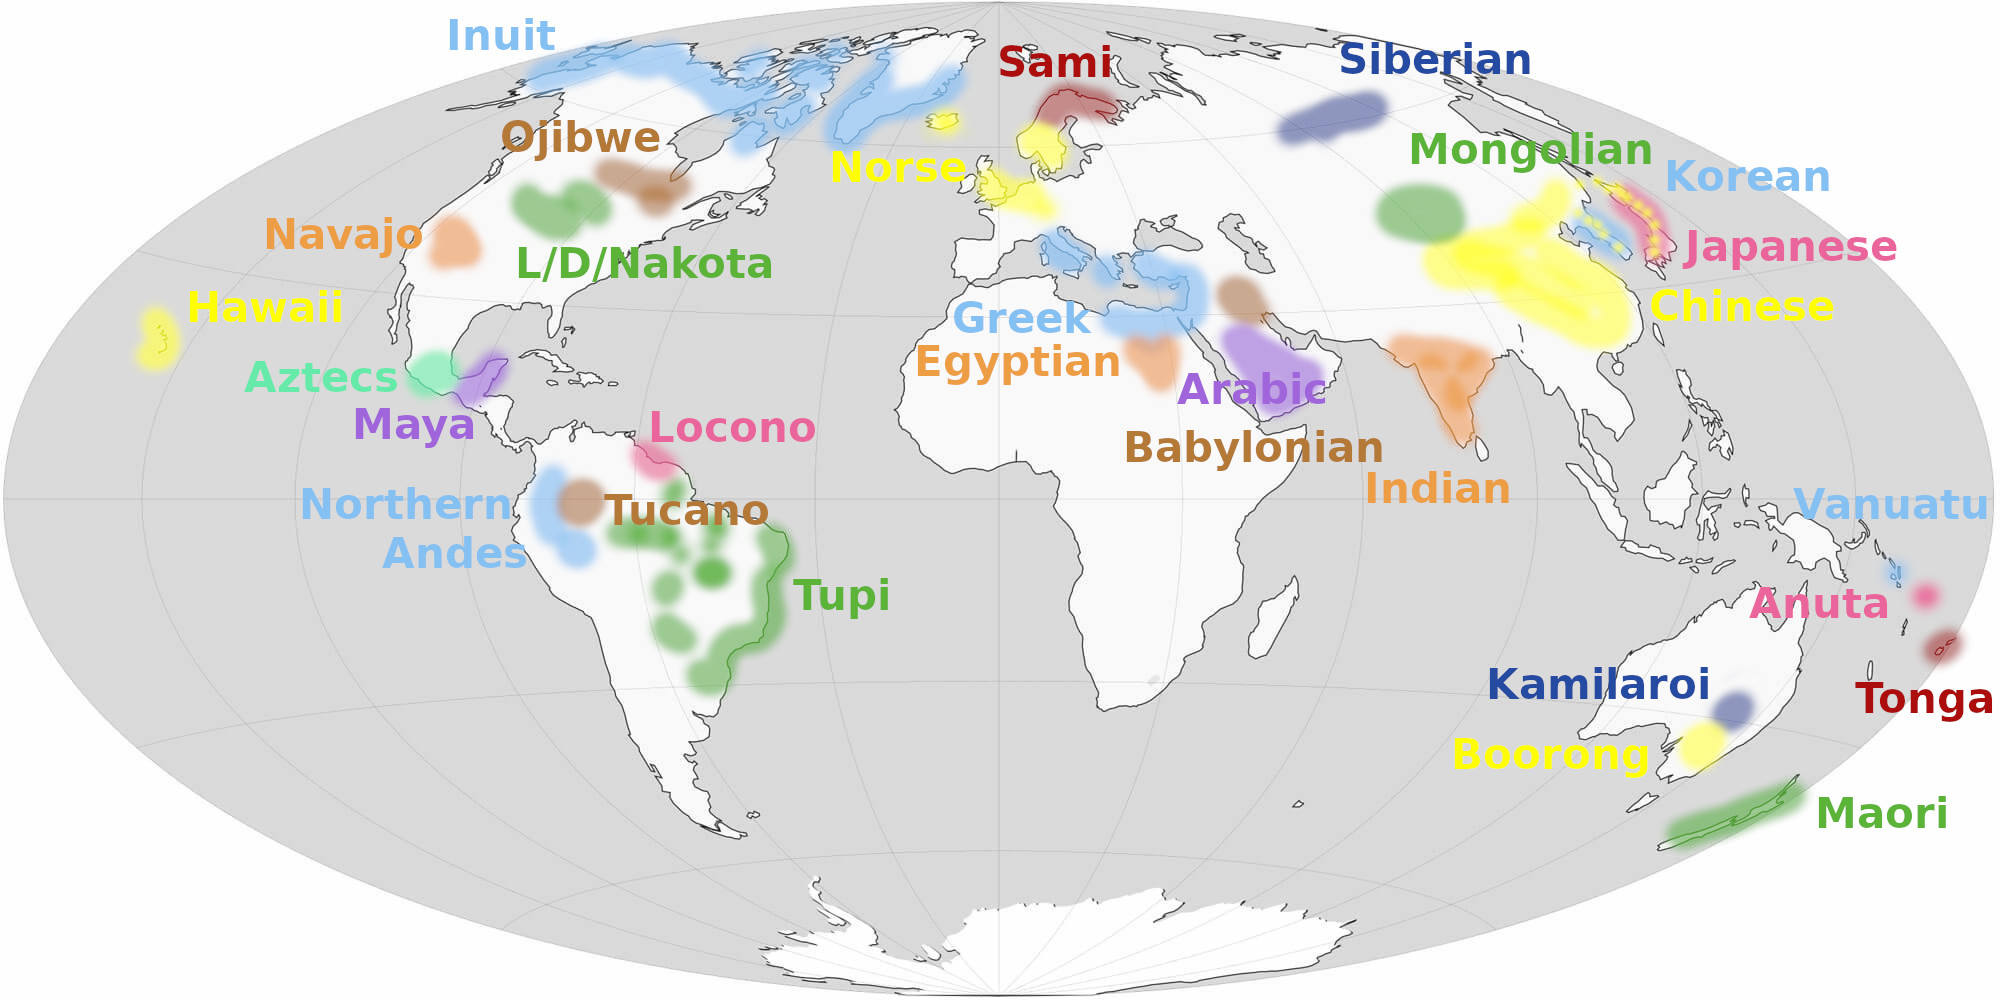
\includegraphics[width=\textwidth]{stellarium-skycultures-map.jpg}
\caption{World map showing Stellarium's built-in set of
  skycultures. To avoid overcrowding, smaller European skycultures
  which are mostly derivatives of the ``Western'' skyculture are not
  shown. (Image: S. M. Hoffmann)}
\label{fig:skycultures}
\end{figure}


\noindent Stellarium comes with a nice set of skycultures from all
over the world (Fig.~\ref{fig:skycultures}). For ethnographers or
historians of science it may be a worthwhile consideration to
illustrate the sky culture of the people they are studying. It is not
very hard to do so, but depending on your data, may require some
skills in image processing.

Some features regarding translation and multilinguality have evolved
over the years, and not all skycultures currently included in
Stellarium adhere to the standards described in the following
sections. Skycultures will also see continuous development in the
coming versions. If you add a new skyculture, please adhere to this
description for an optimal result!


In the Stellarium program folder you can see a folder
\file{skycultures}. Let us assume you work on Windows and want to create a
new Skyculture, say, \emph{myCulture}.

You can take the \file{inuit} directory as template to start with. Just copy the folder 
\file{C:\textbackslash{}Program Files\textbackslash{}Stellarium\textbackslash{}skycultures\textbackslash{}inuit} to
\file{C:\textbackslash{}Users\textbackslash{}[YOU]\textbackslash{}AppData\textbackslash{}Roaming\textbackslash{}Stellarium\textbackslash{} skycultures\textbackslash{}myculture}

In the folder you see image files for the constellation artwork, and all
other files with various extensions are text files. 


\section{Basic Information}
\label{sec:skycultures:info.ini}


In \file{myculture\textbackslash{}info.ini}, change the entries to 
\begin{configfile}
[info]
name=myCulture
author=me
boundaries=none
classification=personal
\end{configfile}

\noindent (or what seems best for you). The name is used for the list entry in
the Starlore tab in the View dialog (see \ref{sec:gui:view:starlore}).

\paragraph{boundaries}
The option ``boundaries'' is optional and may contain the follow values:
\begin{description}
\item[none] --- this value is enabled by default and it designates that this culture doesn't have boundaries of constellations.
\item[iau] --- use this value for variants of ``western'' cultures to enable using default (IAU) boundaries.
\item[own] --- please use it for culture who has own set of boundaries for constellations.
\end{description}

\paragraph{classification}
The option ``classification'' is also optional. \newFeature{0.19.0} It allows some form of quality control:
\begin{description}
  \item[personal] -- this is a personally developed skyculture which
    is not founded in published historical or ethnological research. Stellarium
    may include it when it is ``pretty enough'' without really
    approving its contents.
  \item[traditional] -- (default value) content represents ``common'' knowledge by
    several members of an ethnic community, and the skyculture has
    been developed by members of such community. Our ``Western''
    skyculture is a key example: it has evolved for about 2500 years,
    and modern astronomers use it.
  \item[ethnographic] -- provided by ethnographic researchers based on
    interviews of indigenous people.
  \item[historical] -- based on historical written sources from a
    (usually short) period of the past.
  \item[single] -- represents a single source like a historical atlas,
    or publications of a single author.
  \item[comparative] -- special-purpose compositions \newFeature{0.21.2} of e.g.\ artwork
    from one and stick figures from another skyculture, and optionally
    asterisms as representations of a third. Or comparison of two
    stick figure sets in constellations and asterisms. These figures
    sometimes will appear not to fit together well. This may be
    intended, to explain and highlight just those differences! The
    description text must clearly explain and identify all sources and
    how these differences should be interpreted.
\end{description}

%The classification may show overlaps. Currently (V0.19.0) it is not displayed or evaluated, but will be used in future versions. 

\section{Skyculture Description Files}
\label{sec:skycultures:description}


In order to have translated texts we have files
\file{description.<LANG>.utf8}, where \file{<LANG>} is the two-letter
ISO~639-1 language code, or its extension which contains language and
country code, like \file{pt\_BR} for Brazilian Portuguese. A minimum
skyculture must contain the file \file{description.en.utf8}, this is
\texttt{en=English} text with optional HTML tags for sections, tables,
etc. You can also have embedded images in the HTML (your book cover?
Views of sacred landscapes/buildings/artwork/\ldots?), just make them
PNG format please. The length of the description texts is not limited,
you have room for a good description, tables of names/translations,
links to external resources, whatever seems suitable. When you started
from a copied skyculture, delete the other \file{description.*.utf8}
files.

If you can provide other languages supported by Stellarium, you can
provide translations yourself, else Stellarium translators \emph{may}
translate the English version for you. (It may take years though.) The file
ending \file{.utf8} indicates that for special characters like ÄÖÜßáé
you should use UTF8 encoding. If you write only English/ASCII, this may not
be relevant.

\section{Constellation Names}
\label{sec:skycultures:constellations}

The native constellations are listed in
\file{constellation\_names.eng.fab}. It consists of 3 simple columns:
Abbreviation (or just a serial number), native name, and English
translation. The writing \texttt{\_("name")} allows automatic
translation of the English strings to other languages. These strings
will be used as constellation labels.

You can \newFeature{0.19.2} add a reference comment after each
3-column entry. Just add a white-space, and then a comma-separated list
of numerical references to the books listed in \file{reference.fab}.

The first column (abbreviation) in the Western sky culture provides
the canonical 3-letter abbreviation for constellations as used by the
International Astronomical Union. Such abbreviations may not be
available for the skyculture you are working with, so you must invent
your own. These abbreviations are used as keys in the other files, so
they must be unique within your skyculture.
It is not necessary to have 3-letter keys. 

The keys can be displayed on screen when labels are requested in the
Starlore GUI (section~\ref{sec:gui:view:starlore}). If you want to prevent
certain abbreviations from being displayed, let them start with a
dot. See the effect in the \file{Western (H.A.Rey)} skyculture: In
\menu{Abbreviated} mode, only the official abbreviations are
displayed. In \menu{Native} mode, the second column of
\file{constellation\_names.eng.fab} is shown. Only with setting
\menu{Translated}, the text translated from the text shown in the
third column is shown. If your skyculture is a variant of the Western
skyculture, please use the canonical Latin names, they have all been translated already.

If your skyculture is not a variant of the generally known Western
skyculture, please include an English translation to the name given in
the native language. Else translators will not be able to translate
the name. See a good example in the Mongolian skyculture.

\section{Star Names}
\label{sec:skycultures:starnames}

The file \file{star\_names.fab} contains a list of HIP catalog
numbers and common names for those stars. Each line of the file
contains one record of two fields (separated by the pipe character
(\texttt{|})) or three fields (the first pair is separated by the 
pipe character (\texttt{|}) and the last one separated by the space 
character). The first field is the Hipparcos catalog number of the
star, the second is the common name of the star in a format that enables
translation support, the third is an optional list of references (see \ref{sec:skycultures:references})  
to the source of the information about this name, e.g:
\begin{configfile}
# Piscis Austrinus (PsA)
113368|_("Fomalhaut") 1,2,6,11,12
113368|_("Thalim")
\end{configfile}

In the sample you can see 3 lines: the first line is a comment, the 
second line has 3 fields and the third line has 2 fields. Both lines 
with data have the same Hipparcos number of the star --- \textit{Fomalhaut} is 
the well-known name of HIP 113368, and \textit{Thalim} is an additional 
(not well-known) name of this star.

\section{Planet Names}
\label{sec:skycultures:planetnames}

The file \file{planet\_names.fab} contains a list of native names of
the planets. Each line of the file contains one record of 3 fields,
separated by the white space or tab character. The first field is the
English name of the planet, the second is the native name of the
planet (can be in the native language, but please for maximum
utability use an English transliteration) and the third is the
translatable version of the native name of the planet (translated into
English). Here is an example from the Egyptian skyculture:

\begin{configfile}
Mars	"Horus-Desher"	_("Red Horus")
\end{configfile}

\section{Deep-Sky Objects Names}
\label{sec:skycultures:dsonames}

\noindent\newFeature{0.15.1}The file \file{dso\_names.fab} contains a list of native names for
deep-sky objects (DSO). The format of this file is similar to the 
\file{star\_names.fab} format (see \ref{sec:skycultures:starnames}).
Each line of the file contains one record of two fields (separated 
by the pipe character (\texttt{|})) or three fields (first pair is 
separated by the pipe character (\texttt{|}) and the last one separated 
by the space character). The first field is an identifier of the
deep-sky object, the second is the native name of the DSO in a 
format that enables translation support, the optional third is a  
list of references (see \ref{sec:skycultures:references}) to the source 
of the information about this name, e.g.:
\begin{configfile}
PGC 17223|_("Native name for LMC") 1,2,3
NGC 292  |_("Native name for SMC") 1,3
NGC 292  |_("Small Magellanic Cloud")
\end{configfile}

\section{Stick Figures}
\label{sec:skycultures:stickfigures}

The modern-style stick figures are coded in \file{constellationship.fab}. Lines
look like:

\begin{configfile}
Abbr pairs pair1_star1 pair1_star2 pair2_star1 pair2_star2 ...
\end{configfile}
In this file,
\begin{description}
\item[Abbr] is the abbreviation defined in \file{constellation\_names.eng.fab}
\item[pairs] is the number of line pairs which follow.
\item[pairN\_starA] Hipparcos numbers for the stars which form the
  constellation stick figure. We need two entries per line, longer
  line segments are not supported. To find the HIP number, just have
  Stellarium open and click on the star in Stellarium while editing
  this file.
\end{description}
Anything after the last star number is currently ignored.
Comments can be given in lines starting with \texttt{\#} signs. Empty lines are ignored.

\section{Constellation Boundaries}
\label{sec:skycultures:boundaries}

The optional file\footnote{Please define \texttt{boundaries = own} in the file \file{info.ini} to enable using custom boundaries.} 
\file{constellation\_boundaries.dat} includes data for the boundary lines drawn between constellations. 
The default boundaries for western constellations are defined in the \file{data/constellation\_boundaries.dat} file.

The format for this file is a bit more difficult than the other files. It contains sections which may consist of multiple lines, of the format:

\begin{configfile}
N RA_1 DE_1 RA_2 DE_2 ... RA_N DE_N 2 CON1 CON2
\end{configfile}
where
\begin{description}
\item[N] number of segments for boundary
\item[RA\_n, DE\_n] right ascension (decimal hours) and declination (decimal degrees) of the points of segments in J2000 coordinates.
\item[2 CON1 CON2] this data indicate ``border between 2 constellations CON1 and CON2''. 
      They are used to define isolated boundaries for each constellation (for proper working of the \menu{Select single constellation} option). 
\end{description}

\section{Constellation Artwork}
\label{sec:skycultures:artwork}

Constellation artwork is optional, but may give your skyculture the
final touch, if it requires artwork at all. E.g., H. A. Rey's variant
of the Western skyculture deliberately does not contain artwork.

Each constellation artwork is linked to 3 stars in its constellation. This
is programmed in the file \file{constellationsart.fab}. You have to write lines

\begin{configfile}
  Abbr image_name.png x1 y1 HIP1 x2 y2 HIP2 x3 y3 HIP3
\end{configfile}
where 
\begin{description}
\item[Abbr] is the abbreviation defined in \file{constellation\_names.eng.fab}
\item[image\_name.png] is the file name of your texture. It should be
  sized in a power of two, like $512\times512$, $1024\times2048$
  etc. Avoid dimensions larger than 2048, they are not supported on
  all systems. You can distort images to better exploit the pixels,
  the texture will be stretched back. The background of the artwork
  image must be absolutely black.
\item[x\textit{n}, y\textit{n}, HIP\textit{n}] ($n\in[1, 2, 3]$) pixel locations of the
  star in the constellation drawing (find those in any image editor)
  and HIP\textit{n} is the star number in the Hipparcos catalog, which
  you find when you click on the star in Stellarium.
\end{description}

In case the artwork is only available in a certain projection (e.g.,
an all-sky map), or is otherwise heavily distorted so that the match
is not satisfactory, you may have to re-project the image somehow. For
aligning, you should switch Stellarium to Stereographic projection for
optimal results.

You don't have to shutdown and restart Stellarium during
creation/matching, just switch skyculture to something else and back
to the new one to reload.

\section{Seasonal Rules}
\label{sec:skycultures:seasonal_rules}

File \file{seasonal\_rules.fab} (optional) contains possible seasonal rules for
the visibility of constellations. There is one rule per line. Each
rule contains three elements separated with white space (or tab
character): constellation ID, start of visibility (month) and end of
visibility (month), e.g:

\begin{configfile}
  Emu 6 3
\end{configfile}

\noindent This specifies that constellation Emu (abbreviated also as ``Emu'') is
visible only from June to March.
%% TODO: This feature may need rework. Where is it used?

\section{References}
\label{sec:skycultures:references}

\noindent\newFeature{0.15.1}The file \file{reference.fab} contains a list of information sources. 
Each line of the file contains one record of 3 fields,
separated by the pipe character (\texttt{|}) --- number of source, 
description of source and optional URL, e.g.:

\begin{configfile}
9|Kruger 60|https://en.wikipedia.org/wiki/Kruger_60
\end{configfile}

This file will be used in future versions. It is most important for ``traditional'' 
skycultures collected from various sources to provide traceable references. 

\section{Asterisms and help rays}
\label{sec:skycultures:asterisms}

\noindent\newFeature{0.16.1}Sometimes there is a need to extract some part of a 
constellation into a figure in its own right, or to merge parts from different 
constellations into one big figure --- e.g. ``Big Dipper'' as part of Ursa Major or the 
``Summer Triangle'' consisting of 3 stars from the constellations Cygnus, Lyra and Aquila. 
Those features are called ``asterisms''. 

Other simple figures might be used as navigation helpers --- the help rays. 
As example to help in orientation in the sky the additional lines between constellations 
Ursa Major, Ursa Minor and Cassiopeia might be useful. The asterisms and help rays are listed in
\file{asterism\_names.eng.fab}. This file consists of 2 simple columns:
Abbreviation (or just a serial number) and English
name of asterism. The writing \texttt{\_("name", "asterism")} allows automatic, context sensitive
translation of the English strings to other languages. These strings
will be used as asterisms labels. In addition, after a hash mark (\texttt{\#}) marking a comment sign, 
some reference information can be added in comment lines, like ``List found at \ldots''.
Also, you can \newFeature{0.19.2} again add a reference comment after each
2-column entry. Just add a white-space, and then a comma-separated list
of numerical references to the books listed in \file{reference.fab}.
Collecting sources and giving such references 
is always a good idea. Some later versions of Stellarium may use and display this information.

The stick figures of asterisms are coded in \file{asterism\_lines.fab}
which looks similar to the entries for the constellation
figures. Lines look like:

\begin{configfile}
Abbr type pairs pair1_star1 pair1_star2 pair2_star1 pair2_star2 ...
\end{configfile}
or
\begin{configfile}
Abbr 2 pairs pair1_RA1 pair1_DE1 pair1_RA2 pair1_DE2 pair2_RA1 ...
\end{configfile}
In this file,
\begin{description}
\item[Abbr] is the abbreviation defined in \file{asterism\_names.eng.fab}
\item[type] is the type of line. Use 1 or 2 to define an asterism and 0 for the help rays (0 and 1 uses HIP numbers, and 2 uses coordinates).
\item[pairs] is the number of line pairs which follow.
\item[pairN\_starA] Hipparcos numbers for the stars which form the asterism/help ray stick figure (similar to constellations),
  or equatorial coordinates for epoch J2000.0 of the stars (decimal hours for right ascension and decimal degrees for declination).
  The help rays are actually a special form of asterisms in Stellarium. 
\end{description}

\section{Publish Your Work}
\label{sec:skyculture:publish}

If you are willing to let other users enjoy the result of your hard
work (and we certainly hope you do!), when you are done, please write
a note in the Forum or at GitHub. We will decide about acceptability
and classification, and may ask for better descriptions for the
benefit of our users.

Please be prepared to put the imagery and text
under some compatible open-source license (Creative Commons). Else the
skyculture cannot be hosted by us.
While we cannot be held responsible for legal problems, it seems that
CC BY 4.0
International\footnote{\url{https://creativecommons.org/licenses/by/4.0/}}
or CC BY-SA 4.0
International\footnote{\url{https://creativecommons.org/licenses/by-sa/4.0/}}
licenses are best suited.


%%% Local Variables: 
%%% mode: latex
%%% TeX-master: "guide"
%%% End: 

